\documentclass[10pt]{beamer}

\usetheme[progressbar=frametitle]{metropolis}
\usepackage{appendixnumberbeamer}
\usepackage{subfigure}
\usepackage{booktabs}
\usepackage{varwidth}
\usepackage[scale=2]{ccicons}
\usepackage{svg}
\usepackage{pgfplots}
\newcommand\scalemath[2]{\scalebox{#1}{\mbox{\ensuremath{\displaystyle #2}}}}
\usepackage{xspace}
\usepackage{tikz}
\usetikzlibrary{quantikz}

\newcommand*{\Scale}[2][4]{\scalebox{#1}{$#2$}}%
\newcommand*{\Resize}[2]{\resizebox{#1}{!}{$#2$}}%
\newcommand{\modM}[0]{\,(\text{mod } M)}
\newcommand{\horiz}[0]{\ket{\rightarrow}}
\newcommand{\verti}[0]{\ket{\uparrow}}

\title{QUANTUM BUILDING BLOCKS}
\subtitle{Recap}
\date{\today}
\author{Ulan Seitkaliyev, QSIURP 2022}
\institute{Carnegie Mellon University in Qatar}

\begin{document}

\maketitle

% % Outline frame
% \begin{frame}{Outline}
%     \tableofcontents[hideallsubsections]
% \end{frame}

\section[Single-Qubit Quantum Systems]{Single-Qubit Quantum Systems}

\begin{frame}[fragile]{The Quantum Mechanics of Photon Polarization}
    There is a simple experiment with light polarization illustrates some of the \textbf{nonintuitive} behavior of quantum systems, behavior that is \textbf{exploited} to good effect in quantum algorithms and protocols. 

\end{frame}

\begin{frame}[fragile]{The Quantum Mechanics of Photon Polarization}
    Shine a beam of light on a projection screen. When polaroid \textbf{A} is placed between the light source and the screen, the intensity of the light reaching the screen is \textbf{reduced}.
    
    \begin{figure}[htbp]
          \centering
          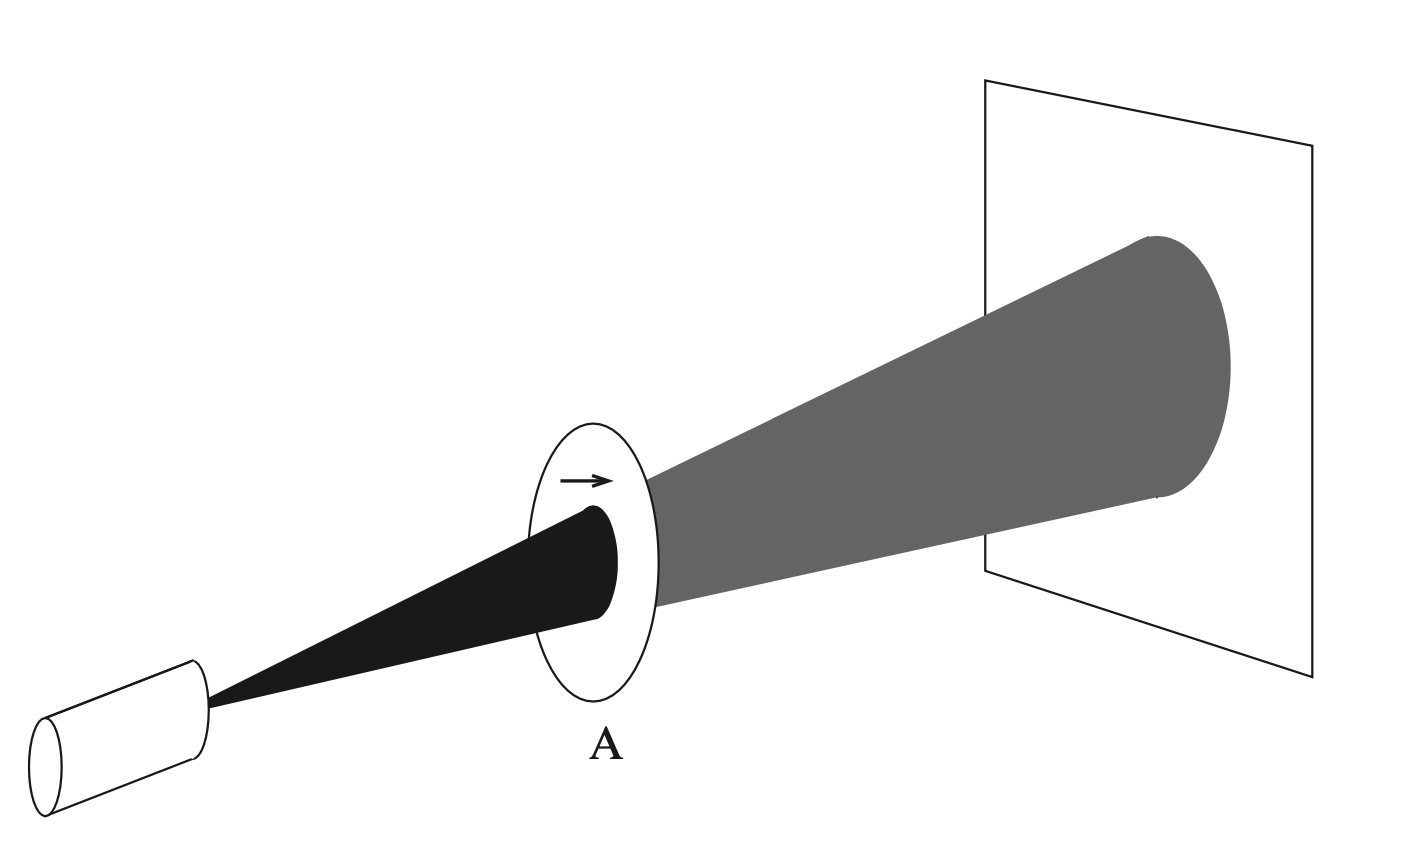
\includegraphics[width=0.8\textwidth]{h.png}
          \caption{Single polaroid weaken unpolarized light by 50 percent.}
    \end{figure}
    
\end{frame}

\begin{frame}[fragile]{The Quantum Mechanics of Photon Polarization}
    Next, if we place polaroid \textbf{C} and if polaroid C is rotated so that its polarization is orthogonal (vertical) to the polarization of \textbf{A}, no light reaches the screen.
    \begin{figure}[htbp]
          \centering
          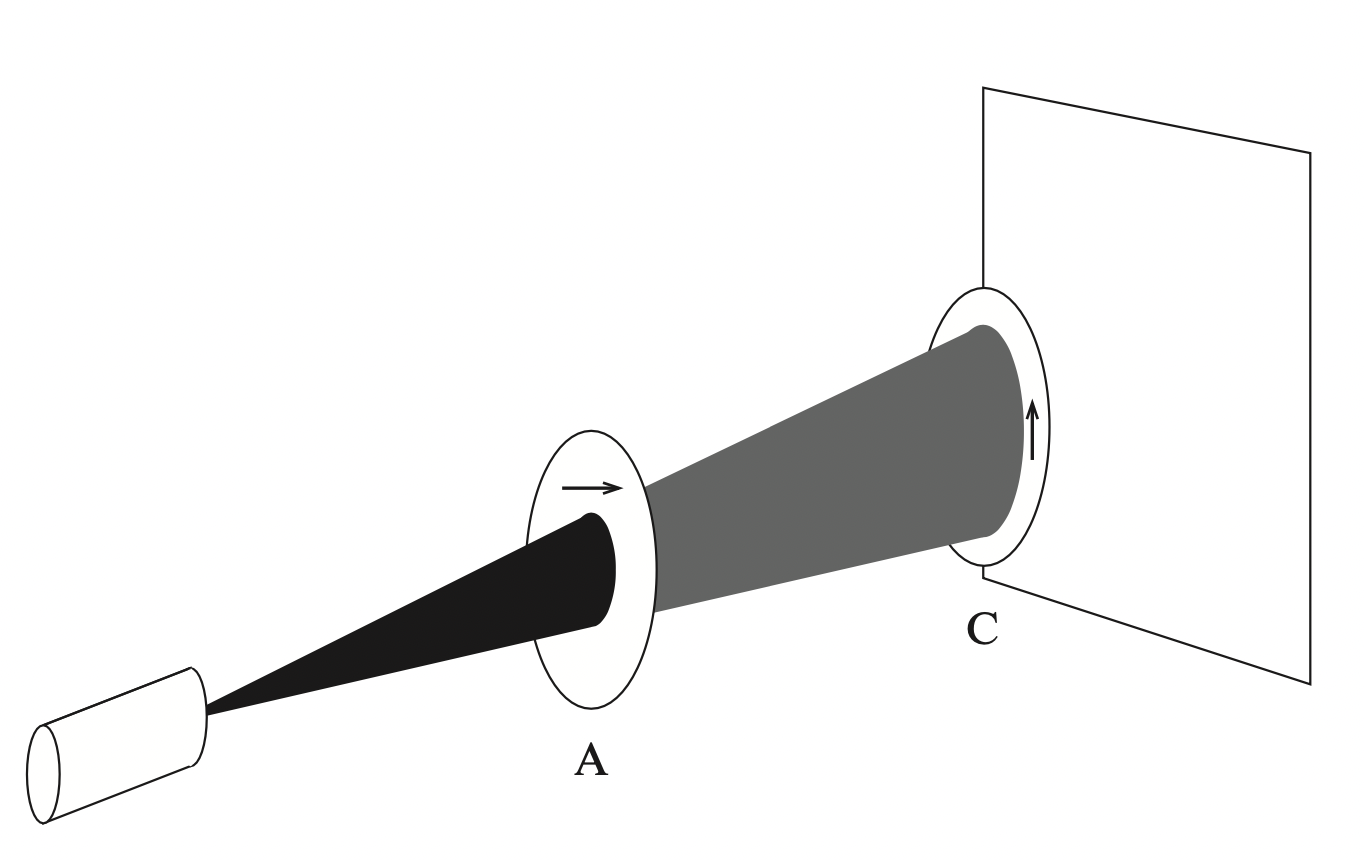
\includegraphics[width=0.8\textwidth]{hv.png}
          \caption{Two orthogonal polaroids block all photons.}
    \end{figure}
    
\end{frame}

\begin{frame}[fragile]{The Quantum Mechanics of Photon Polarization}
    Finally, place polaroid \textbf{B} between polaroids \textbf{A} and \textbf{C}. Surprisingly, at most polarization angles of \textbf{B}, light shines on the screen. The intensity of this light will be maximal if the polarization of \textbf{B} is at $45^{\circ}$ to both \textbf{A} and \textbf{C}.
    \begin{figure}[htbp]
          \centering
          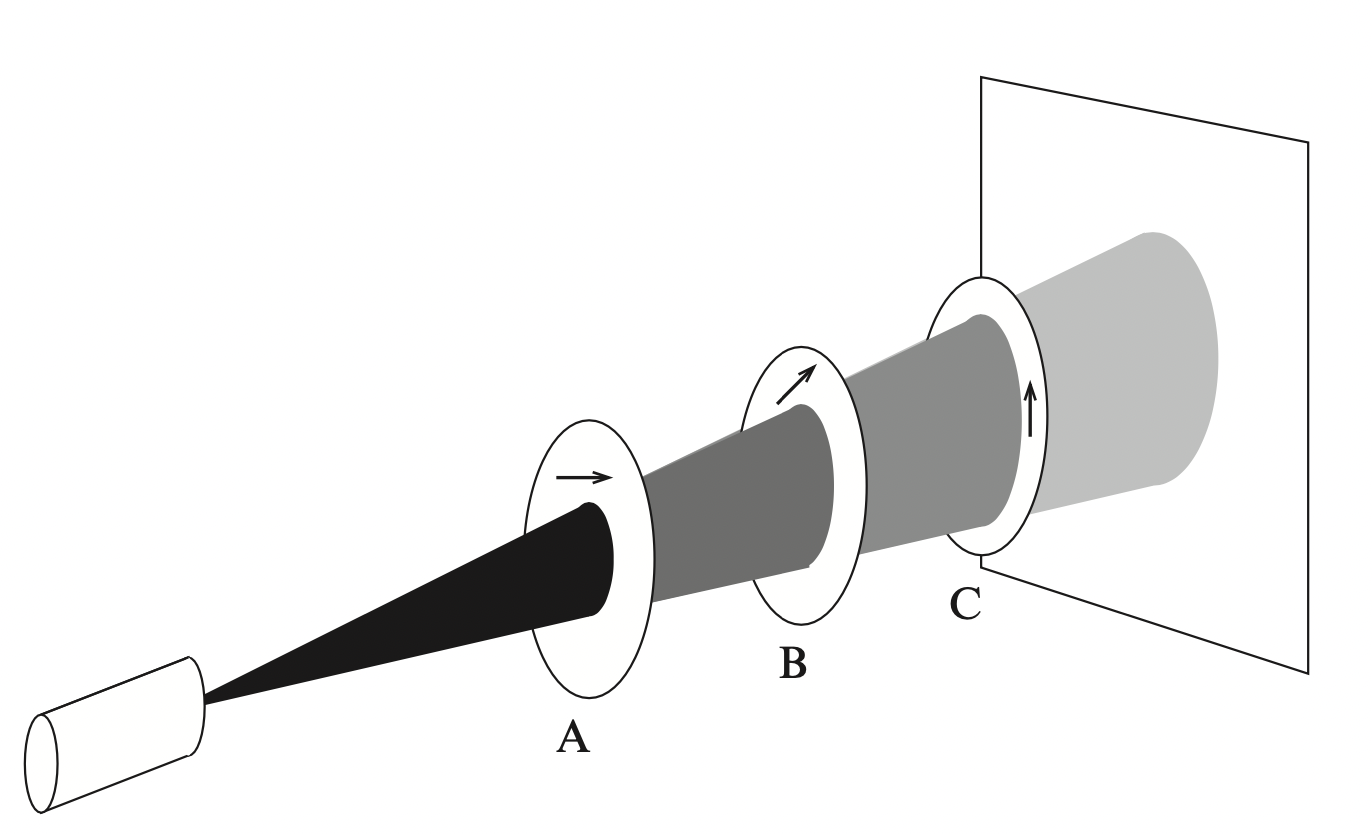
\includegraphics[width=0.8\textwidth]{hdv.png}
          \caption{Inserting a third polaroid allows photons to pass.}
    \end{figure}
\end{frame}

\begin{frame}[fragile]{The Quantum Mechanics of Photon Polarization}
    Clearly the polaroids cannot be acting as \textbf{simple sieves}; otherwise, inserting polaroid B could not increase the number of photons reaching the screen.
\end{frame}

\begin{frame}[fragile]{Some notation before an explanation}
        % $\horiz$ and $\verti$
        Quantum mechanics models a photon’s polarization state by a unit vector, a vector of length $1$, pointing in the appropriate direction.
        
        We write $\verti$ and $\horiz$ for the unit vectors that represent vertical and horizontal polarization respectively.
        
        In quantum mechanics, the standard notation for a vector representing a quantum state is $\ket{v}$, just as $\vec{v}$ or \textbf{v} are notations used for vectors in other settings.
        
        An arbitrary polarization can be expressed as a linear combination $$\ket{v} = a\verti + b\horiz$$ of the two basis vectors $\verti$ and $\horiz$.
\end{frame}

\begin{frame}[fragile]{Polaroid interacts with a photon}
    When a photon with polarization $\ket{v} = a\verti + b\horiz$ meets a polaroid with preferred axis $\verti$, the photon will get through with probability $|a|^2$ and will be absorbed with probability $|b|^2$.

    Any photon that passes through the polaroid will now be polarized in the direction of the polaroid’s preferred axis. 
    
\end{frame}

\begin{frame}[fragile]{A Quantum Explanation}


        In the experiment, any photons that pass through polaroid \textbf{A}, will leave as a $\horiz$. 
        
        So it has no chance of passing through polaroid \textbf{C}, which was vertical.
        
        To understand what will happen, when we insert \textbf{B}, let's rewrite 
        $$\horiz = \frac{1}{\sqrt{2}} \ket{\nearrow} - \frac{1}{\sqrt{2}} \ket{\nwarrow}.$$
        
        So, any photon in $\horiz$ state will have a $\frac{1}{\sqrt{2}}$ amplitude in $\ket{\nearrow}$ direction. Thus, it has a probability of $\frac{1}{2}$ passing through \textbf{B}.
        
        The same happens with \textbf{C} as
        $$\ket{\nearrow} = \frac{1}{\sqrt{2}} \verti + \frac{1}{\sqrt{2}} \horiz.$$
\end{frame}

\begin{frame}[fragile]{The Quantum Mechanics of Photon Polarization}
    We see how the model explains that $\frac{1}{8}$ of light pass through \textbf{A, B, C}.
    \begin{figure}[htbp]
          \centering
          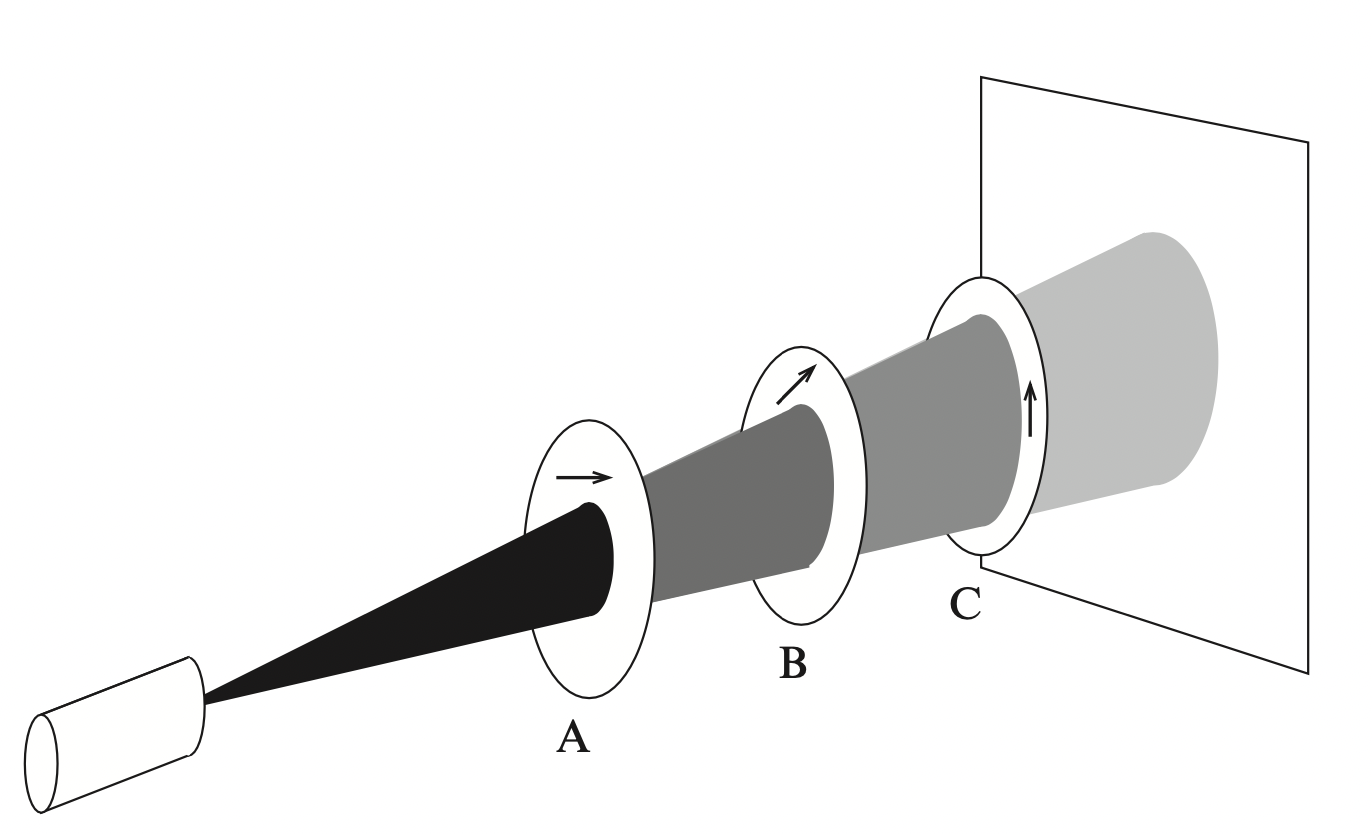
\includegraphics[width=0.8\textwidth]{hdv.png}
    \end{figure}
\end{frame}

\begin{frame}[fragile]{Single Quantum Bits}
The space of possible polarization states of a photon is an example of a quantum bit, or \textbf{qubit}. A qubit has a continuum of possible values: any state represented by a unit vector $a\verti + b\horiz$ is a legitimate qubit value.

Any quantum mechanical system that can be modeled by a two-dimensional complex vector space can be viewed as a qubit. 

It~includes photon polarization, electron spin, and the ground state together with an excited state of an atom.

It is as yet unclear which two-state systems will be most suitable for physical realizations of quantum computers; it is likely that a \textbf{variety of physical representation} of qubits will be used.
\end{frame}

\begin{frame}[fragile]{$\ket{0}$ and $\ket{1}$}
We just need to specify any two orthonormal (perpendicular) states and call them $\ket{0}$ and $\ket{1}$. It can be any states. For example in the photon polarization example we could equally set $\{\ket{0}, \ket{1}\} = \{\horiz, \verti\}$ or $\{\ket{0}, \ket{1}\} = \{\ket{\nearrow}, \ket{\nwarrow}\}.$

We will use the convention that $\ket{0} = \verti, \ket{1} = \horiz$, which means $\ket{\nearrow} = \frac{1}{\sqrt{2}} \left(\ket{0} + \ket{1}\right)$  and $\ket{\nwarrow} = \frac{1}{\sqrt{2}} \left(\ket{0} - \ket{1}\right)$.


We will call $\{\ket{0}, \ket{1}\}$ as standard basis. 

And write any qubit in the state $a\ket{0} + b\ket{1}$ as $\begin{pmatrix}
a \\ b
\end{pmatrix}.$
\end{frame}


\begin{frame}[fragile]{Single-Qubit Measurement}
    Quantum theory postulates that any device that measures a two-state quantum system must have two preferred states whose representative vectors, $\{\ket{u}, \ket{u^{\perp}}\}$, form an \textbf{orthonormal} basis for the associated vector space.
    
    The probability of measuring $\ket{u}$ or $\ket{u^{\perp}}$ is equal to the square of the magnitude of $\ket{u}$ and $\ket{u^{\perp}}$, respectively. 
    
    And measured qubit has to gain amplitude of 1 in the measured state, so the measurement outcome is always one of the two basis vectors.
    
    This behavior of measurement is an \textbf{axiom} of quantum mechanics.
    
    For this reason, whenever we say \textit{“measure a qubit,"} we must specify with respect to which basis the measurement takes place.
\end{frame}

\begin{frame}[fragile]{Pop-science misconception: $\ket{v}$ is not prob. mix of $\ket{0}, \ket{1}$}

Rather, $\ket{v}$ is a definite state, which, when measured in certain bases, gives deterministic results, but for some other bases gives random results. 

For example a state $$\ket{\nearrow} = \frac{1}{\sqrt{2}} \left(\horiz + \verti \right)$$ is deterministic in Hadamard basis $\{\ket{\nearrow}, \ket{\nwarrow}\}$, however random in $\{\horiz, \verti\}$.

It is OK to think that $a\ket{0} + b\ket{1}$ is at the same time $\ket{0}, \ket{1}$, however we have to be careful to distinguish between $$\ket{+} = \frac{1}{\sqrt{2}}\left(\ket{0} + \ket{1}\right),\,\ket{-} = \frac{1}{\sqrt{2}}\left(\ket{0} - \ket{1}\right)\, \text{ and } \ket{i} = \frac{1}{\sqrt{2}}\left(\ket{0} + i\ket{1}\right)$$ that behave differently in many cases, yet have the same proportion of $\ket{0}$ and $\ket{1}$ .
\end{frame}

\begin{frame}[fragile]{A global phase vs relative phase} 
    Let's consider a qubit state $\ket{1}$, $-\ket{1}$, and $i\ket{1}$. Can we differentiate them? 
    
    Our measuring devices can not. This is what we call a global phase. We can not tell a difference between states $\ket{\phi}$ and $c \cdot \ket{\phi}$, when $|c| = 1$ in other symbols, $(c = e^{i\theta}$ for some $\theta)$.
    
    We only care the difference between the given states, their relative phases. 
    
    While multiplication with a unit constant does not change a quantum state vector, relative phases in a superposition do represent distinct quantum states: eventhough $\ket{v_1} \sim e^{i\theta} \ket{v_1}$, $$\frac{1}{\sqrt{2}}\left(\ket{v_1} + \ket{v_2}\right) \not\sim \frac{1}{\sqrt{2}}\left( e^{i\theta} \ket{v_1} + \ket{v_2}\right).$$
    
    
\end{frame}

\begin{frame}[fragile]{Bloch Sphere} 
    It turns out it is also convenient to represent a qubit as a point in a 3 dimensional space, where each diameter is a orthornormal basis of a qubit. Note that the angles are doubled in this representation.
        \begin{figure}[htbp]
          \centering
          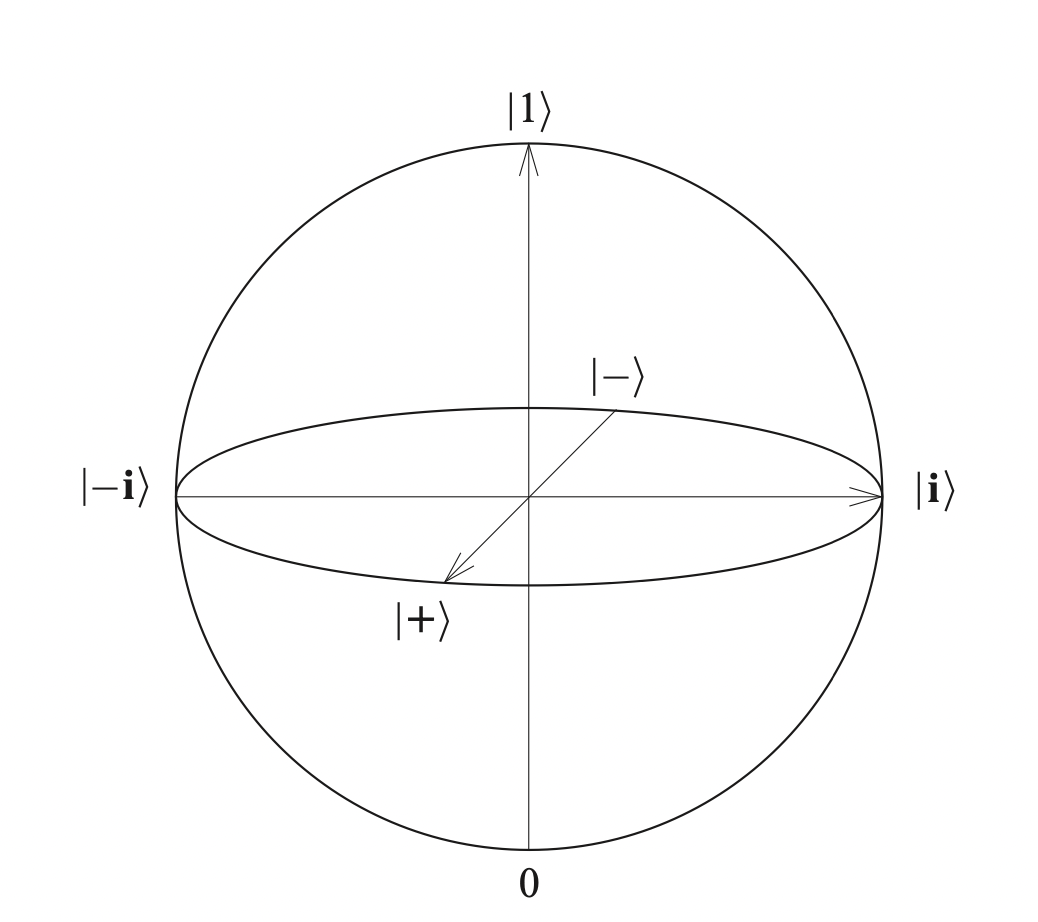
\includegraphics[width=0.5\textwidth]{bloch.png}
          \caption{Location of certain single-qubit states on the surface of the Bloch sphere.}
    \end{figure}
\end{frame}


\end{document}

